\documentclass[a4paper,12pt,titlepage]{article}
\usepackage{fancyhdr}
\usepackage{t1enc}
\usepackage[utf8]{inputenc}
\usepackage[magyar]{babel}
\usepackage{lmodern}
\usepackage[pdftex]{graphicx}
\usepackage[lflt]{floatflt}
\usepackage{epstopdf}
\usepackage{amsmath,amssymb}
\usepackage{icomma}
\usepackage{array}
\usepackage[unicode,colorlinks]{hyperref}
\usepackage{fullpage}
\usepackage{booktabs}
\usepackage{subcaption}
\usepackage{mathtools}
\usepackage{physics}
\usepackage{csquotes}

\hypersetup{allcolors=black}
\hypersetup{pdfstartview=FitH}
\hypersetup{pdfinfo={
	Title={Szupravezetőbeli spin- és töltéskorrelációk elméleti vizsgálata},
	Author={},
	Subject={},
	Keywords={}
}}


\title{\bf Szupravezetőbeli spin- és töltéskorrelációk elméleti vizsgálata}
\author{Hajdú Csanád \\ \small Témavezető: Dr.\ Zaránd Gergely Attila}
\date{2021.\ 05.\ 21.}
\topmargin = 0pt
\headheight = 14.5pt
\headsep = 14.5pt

\pagestyle{fancy}
\lhead{\small {{Szupravezetőbeli spin- és töltéskorrelációk elméleti vizsgálata} -- 2021.\ 05.\ 21.}}
\rhead{Hajdú Csanád}

\widowpenalty=10000 \clubpenalty=10000

% taken from https://tex.stackexchange.com/a/175245
\makeatletter
\DeclareRobustCommand*\uell{\mathpalette\@uell\relax}
\newcommand*\@uell[2]{
	% We need to adjust the width of \uell to be the same as \ell
	\setbox0=\hbox{$#1\ell$}
	\setbox1=\hbox{\rotatebox{10}{$#1\ell$}}
	\dimen0=\wd0 \advance\dimen0 by -\wd1 \divide\dimen0 by 2
	\mathord{\lower 0.1ex \hbox{\kern\dimen0\unhbox1\kern\dimen0}}
}

\newcommand{\KK}{{\vb*{k}}}
\newcommand{\LL}{{\vb*{\ell}}}
\newcommand{\RR}{{\vb*{r}}}
\newcommand{\phantomdagger}{{\phantom{\dagger}}}

\begin{document}

\begin{titlepage}
\begin{center}
	\vspace*{1cm}
	\textbf{\huge Szupravezetőbeli spin- és töltéskorrelációk elméleti vizsgálata}

	\vspace{3.5cm}

	\Large
	Hajdú Csanád

	\vspace{2.5cm}
	{\normalsize Témavezető:} \\
	Dr.\ Zaránd Gergely

	\vfill

	BME Természettudományi Kar \\
	Elméleti Fizika Tanszék

	\vspace{1.5cm}

	2021.\ 05.\ 21.

	\begin{figure}[b]
		\centering
		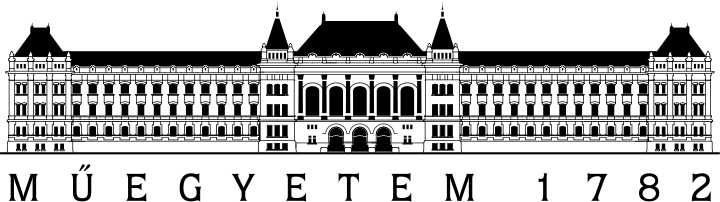
\includegraphics[width=6cm]{bme-logo.png}
	\end{figure}
\end{center}
\end{titlepage}

\tableofcontents \newpage


% ================================================================
\section{Bevezetés}

A szupravezetést a 20.\ század elején fedezve fel Heike Kamerlingh Onnes holland fizikus, amikor a higany ellenállását vizsgálta alacsony hőmérsékleten.  Azt tapasztalta, hogy $4,2$\,K alatt az ellenállás ugrásszerűen nullára csökkent.  Azóta sok más elemi fémnél és ötvözetnél is tapasztaltak szupravezetést.  Mindegyiknél létezik egy $T_\text{c}$ kritikus hőmérséklet, ami alatt a vezető disszipáció nélkül képes áramot vezetni.  A kritikus hőmérséklet értéke jellemzően $10$\,K alatt van, viszont léteznek olyan anyagok is, amik már $100$\,K körül is szupravezetnek.  Az ilyen anyagokat magas hőmérsékletű szupravezetőknek nevezzük.  Utóbbiak nagy előnye, hogy folyékony hélium helyett folyékony nitrogénnel is lehűthetők annyira, hogy szupravezessenek.

\begin{figure}[h!]
	\centering
	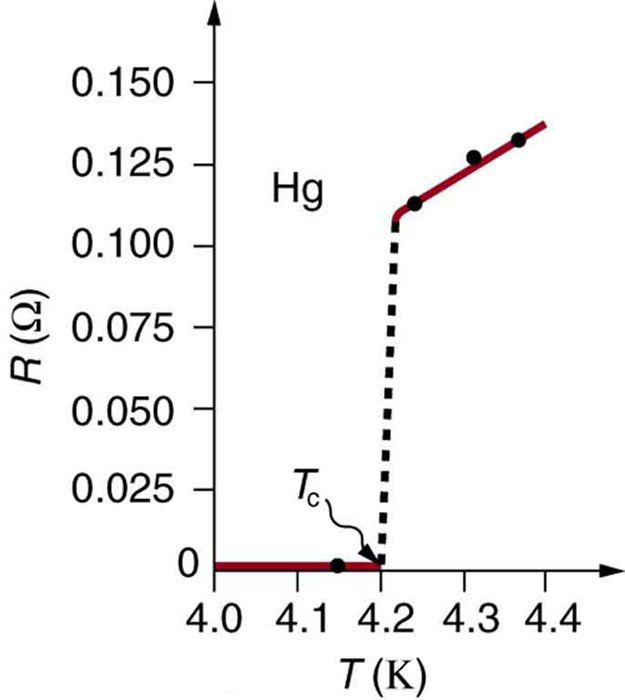
\includegraphics[width=5cm]{higany_R-vs-T.jpg}
	\caption[]{Egy higany minta ellenállása $T_\text{c}$ körül.\footnotemark}
\end{figure}
\footnotetext{\href{https://pressbooks.bccampus.ca/collegephysics/chapter/resistance-and-resistivity/}{\texttt{https://pressbooks.bccampus.ca/collegephysics/chapter/resistance-and-resistivity/}}}

A szupravezetés jelenségének fontos tulajdonsága a Meissner-effektus, ami egy minta belsejében a mágneses tér teljes kiszorítását jelenti.  Könnyen belátható, hogy egy ideális vezető belsejében a mágneses tér erőssége állandó, a Meissner-effektus viszont ennél nagyobb megszorítást jelent: a minta belsejében a mágneses tér állandó és zérus, még akkor is, ha a szupravezető állapotra egy külső mágneses tér mellett hűtjük le a mintát.

A szupravezetőket széles körben használják.  Az egyik alapvető jelenség, amit felhasználnak a Josephson-effektus, ahol két szupravezető rész közé egy vékony szigetelőt illesztenek és a két vezetőre egy egyenfeszültséget kapcsolnak.  Ekkor a mintán váltóáram mérhető, aminek a frekvenciája $\omega_\text{J} = \frac{2e V}{\hbar}$.  Egy ilyen Josephson-átmenetet használ az úgynevezett SQUID is (superconducting quantum interference device), amivel mágneses tereket lehet nagy pontossággal mérni.  Ezen kívül a Josephson-effektus alapján definiálják az SI rendszerben a volt egységét.  A szupravezetésnek fontos felhasználási területe a nagyterű szupravezető mágnesek, amiket többek között az orvostudományban is használnak MRI készülékekben.  Kvantumszámítógépekben is előnyös szupravezetőket használni a kvantumbitekhez, mivel az energiaspektrumukban lévő gap védelmet biztosít az alacsonyfrekvenciás zaj ellen.

A felfedezése óta számos elmélet született a szupravezetés jelenségének leírására.  A két meghatározó elmélet a Ginzburg--Landau-elmélet, ami egy fenomenológikus elmélet, illetve a BCS-elmélet, ami egy mikroszkópikus leírást ad.
A Ginzburg--Landau-elméletet 1950-ben dolgozták ki Vitaly Ginzburg\footnote{Vitaly Lazarevich Ginzburg, Nobel-díjas (2003) orosz fizikus} és Lev Landau\footnote{Lev Davidovich Landau, Nobel-díjas (1962) orosz fizikus} orosz fizikusok.  Az elmélet jó leírást ad a szupravezetők makroszkópikus tulajdonságaira még olyan anyagoknál is, amikre a BCS-elmélet nem használható.  Ilyenek például a magas hőmérsékletű szupravezetők és a nehéz fermion rendszerek.  Az elméletből ezen kívül levezethető még az első- és másodfajú szupravezetők megkülönböztetése.

A BCS-elméletet John Bardeen\footnote{John Bardeen, kétszeres Nobel-díjas (1956 és 1972) amerikai mérnök és fizikus}, Leon N.\ Cooper\footnote{Leon N.\ Cooper, Nobel-díjas (1972) amerikai fizikus} és John Robert Schrieffer\footnote{John Robert Schrieffer, Nobel-díjas (1972) amerikai fizikus} amerikai fizikusok dolgozták ki, és publikálták 1957-ben.  A BCS-elmélet egy mikroszkópikus leírásmódot ad a szupravezetés jelenségére.  Az elmélet szerint a vezetési elektronok úgynevezett Cooper-párokat alkotnak a köztük lévő, rácsrezgések által közvetített, vonzó kölcsönhatás miatt.  Először Cooper mutatta meg, hogy akármilyen gyenge vonzó kölcsönhatás mellett is a normál állapot instabil lesz, és az elektronok párokba rendeződnek.  Az elektronok párokba rendeződését mérésekkel is igazolni lehet.  A vezető részecskék töltése, így például a Josephson-frekvenciában szereplő töltés is kétszerese az elektron töltésének.

Szupravezetésnél a minta energiaspektrumában megjelenik egy \enquote{rés}, ez az úgynevezett \emph{szupravezető gap}.  Ez a gap a hőmérséklet csökkenésével nő, és $0$\,K-nél éri el a maximumát.  Kialakulása fontos szerepet játszik a szupravezetésben.  Azt tapasztaljuk, hogy ha a gap-et eltüntetjük például egy erős mágneses térrel, akkor a minta már nem szupravezet.  A szupravezető gap értékének hőmérsékletfüggését a \ref{sc-gap}.\ ábrán láthatjuk.  A gap jelenléte azt is jelenti, hogy kevés termikus gerjesztés van a szupravezető állapotban.

\begin{figure}[h!]
	\centering
	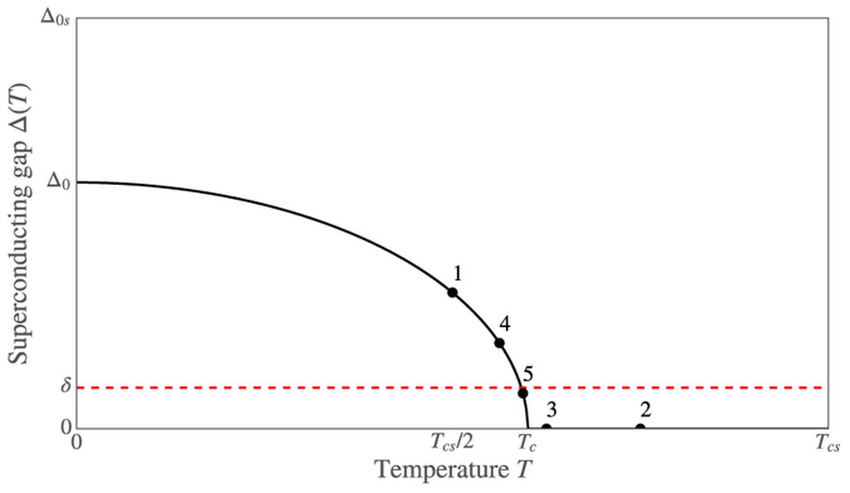
\includegraphics[width=12cm]{sc_gap.png}
	\caption[]{Szupravezető gap a hőmérséklet függvényében.\footnotemark}
	\label{sc-gap}
\end{figure}
\footnotetext{\href{https://www.researchgate.net/figure/Sketch-of-the-superconducting-gap-D-as-a-function-of-temperature-T-for-a-superconducting_fig3_305412985}{\texttt{https://www.researchgate.net/figure/Sketch-of-the-superconducting-gap-D-\\ as-a-function-of-temperature-T-for-a-superconducting\_fig3\_305412985}}}

\newpage

A dolgozat célja az, hogy a szupravezető gap jelenléte mellett vizsgáljuk a spin- és töltéskorrelációs függvényeket, és összehasonlítsuk őket a normál állapotban lévő függvényekkel.  Hosszabb távon cél, hogy megértsük egy szupravezetőbe helyezett mágneses szennyezés körül kialakult úgynevezett Kondo-felhőben a spin-korrelációkat.

A dolgozatban először megnézzük a BCS Hamilton-operátor alakját, majd megmutatjuk, hogy ez transzformálható egy olyan alakra, ahol léptetőoperátorok jelennek meg, majd ezekkel a léptetőoperátorokkal felírjuk a korrelációs függvényeket.  Azt fogjuk látni, hogy ezekben két független függvény jelenik meg, amiket kiszámolunk mind normál állapotban, mind szupravezető állapotban.  Ezen függvények asszimpototikus viselkedését is megvizsgáljuk és analitikus közelítő függvényeket adunk meg közel- és távoltérben.  Végül ezek segítségével megkapjuk a spin- és töltéskorrelációs függvényeket normál- és szupravezető állapotban.

A számolásokhoz alapvető kvantumtérelméleti eszközöket használunk, részecske keltő és eltüntető operátorokat, illetve átlagtér közelítést.  Ezen kívül a BCS-elmélet közelítéseivel is élünk.



% ================================================================
\section{Fizikai modell}

\subsection{A BCS Hamilton-operátor}

A BCS-emélet egy egyszerű átlagtér modellt vesz a szupravezetők leírására.  A Hamilton-operátort két részből építi fel, a $H_0$ kinetikus és a $H_\text{int}$ kölcsönhatási tagokból.  A kinetikus tag
\begin{equation}
	H_0 = \sum\limits_\KK \xi_\KK \left( c_{\KK \uparrow}^\dagger c_{\KK \uparrow} + c_{\KK \downarrow}^\dagger c_{\KK \downarrow} \right),
\end{equation}
ahol $c_{\KK \sigma}^\dagger$ a $\left( \KK \sigma \right)$ sajátállapotú elektron keltő operátora és
$$ \xi_\KK = \frac{\hbar^2 k^2}{2 m} - E_\text{F} $$
az elektron kinetikus energiája a Fermi-energiához viszonyítva.

A kölcsönhatási tagnál azt a közelítést vesszük, hogy az elektronok csak a Cooper-párokon belül hatnak kölcsön.  Így $H_\text{int}$ felírható úgy, mint a Cooper-párok $\left( \KK \uparrow, -\KK \downarrow \right)$ állapotból $\left( \LL \uparrow, -\LL \downarrow \right)$ állapotba való átmenete,
\begin{equation} \label{H-int-def}
	H_\text{int} = \sum\limits_{\KK, \LL} V_{\KK \LL} \, c_{\LL \uparrow}^\dagger c_{-\LL \downarrow}^\dagger c_{-\KK \downarrow} c_{\KK \uparrow},
\end{equation}
ahol $V_{\KK \LL}$ az átmenet valószínűségi amplitúdója.  A BCS-elméletben ezt a valószínűséget úgy választjuk meg, hogy
$$ V_{\KK \LL} = \left\{ \begin{array}{rl}
	-V, & \text{ha } \left| \xi_\LL \right| < \hbar \omega_\text{D} \text{ és } \left| \xi_\KK \right| < \hbar \omega_\text{D} \\
	0, & \text{egyébként}
\end{array} \right. , $$
ahol $\omega_\text{D}$ a Debeye-frekvencia.  Ez azt jelenti, hogy csak a Fermi-felület közelében lévő elektronok hatnak kölcsön, tehát csak ezek lesznek vezető elektronok.

A kölcsönhatási tag alakjának meghatározásához vezessünk be egy variációs hullámyfüggvényt,
\begin{equation} \label{phi-tilde}
	\ket{\tilde{\phi}} \equiv \prod\limits_\KK \left( u_\KK + v_\KK \, c_{\KK \uparrow}^\dagger c_{-\KK \downarrow}^\dagger \right) \ket{0},
\end{equation}
ahol a $\ket{0}$ vákuum állapotba helyezünk be Cooper-párokat valamilyen amplitúdóval.  Az $u_\KK$ és $v_\KK$ együtthatók általános esetben komplexek és ahhoz, hogy $\ket{\tilde{\phi}}$ normálva legyen teljesülnie kell az
\begin{equation} \label{u-v-norm}
	\left| u_\KK \right|^2 + \left| v_\KK \right|^2 = 1
\end{equation}
relációnak.

Ezzel a formalizmussal a normál állapot hullámfüggvényét is felírhatjuk, ahol minden elektronállapot be van töltve a Fermi-felületig,
\begin{equation} \label{u-v-normal}
	\ket{\tilde{\phi}_\text{n}} = \prod\limits_{\left| \KK \right| < k_\text{F}} c_{\KK \uparrow}^\dagger c_{-\KK \downarrow}^\dagger \ket{0},
\end{equation}
ez az
\begin{equation} \label{u-v-sc}
	u_\KK = \left\{ \begin{array}{ll} 0, & \text{ha } \left| \KK \right| < k_\text{F} \\ 1, & \text{ha } \left| \KK \right| > k_\text{F} \end{array} \right.
	~~~ \text{és} ~~~
	v_\KK = \left\{ \begin{array}{ll} 1, & \text{ha } \left| \KK \right| < k_\text{F} \\ 0, & \text{ha } \left| \KK \right| > k_\text{F} \end{array} \right.
\end{equation}
együtthatóknak felel meg.

Vezessük be a $\Delta_\KK$ mennyiséget,
\begin{equation}
	\Delta_\KK^* \equiv \left\{ \begin{array}{ll}
	V \, {\sum\limits_\LL}^\prime \expval{c_{\LL \uparrow}^\dagger c_{-\LL \downarrow}^\dagger}, & \text{ha } \left| \xi_\KK \right| < \hbar \omega_\text{D} \\
	0, & \text{egyébként}
	\end{array} \right. ,
\end{equation}
ahol ${\sum_\LL}^\prime$ azt jelenti, hogy az összegzés csak a $\left| \xi_\LL \right| < \hbar \omega_\text{D}$ állapotokra van.  Ezután egy átlagtér közelítést alkalmazva a \eqref{H-int-def} definícióra azt kapjuk, hogy
\begin{equation}
	H_\text{int} = - \sum\limits_\KK \left( \Delta_\KK c_{\KK \uparrow}^\dagger c_{-\KK \downarrow}^\dagger + \Delta_\KK^* c_{-\KK \downarrow} c_{\KK \uparrow} \right) + \text{cst}.
\end{equation}

Ezzel felírhatjuk a teljes BCS Hamilton-operátort,
\begin{equation}
	H_\text{BCS} = H_0 + H_\text{int} = \sum\limits_\KK \left[ \xi_\KK \left( c_{\KK \uparrow}^\dagger c_{\KK \uparrow} + c_{\KK \downarrow}^\dagger c_{\KK \downarrow} \right) - \Delta_\KK c_{\KK \uparrow}^\dagger c_{-\KK \downarrow}^\dagger - \Delta_\KK^* c_{-\KK \downarrow} c_{\KK \uparrow} \right] + \text{cst}.
\end{equation}


\subsection{Az szupravezető-állapot léptetőoperátorai}

A BCS Hamilton-operátor spektrumának meghatározásához fejezzük ki azt léptetlőoperátorok segítségével,
\begin{equation} \label{H-BCS}
	H_\text{BCS} = \sum\limits_\KK E_\KK \left( \gamma_{\KK \uparrow}^\dagger \gamma_{\KK \uparrow} + \gamma_{\KK \downarrow}^\dagger \gamma_{\KK \downarrow} \right) + \text{cst},
\end{equation}
ahol a $\gamma_{\KK \sigma}$ operátorok a szupravezető-állapot kvázirészecskéinek léptetőoperátorai.  Továbbá igaz rájuk, hogy
\begin{equation} \label{gamma-anticommutator}
\begin{split}
	\anticommutator{\gamma_{\KK \sigma}^\phantomdagger}{\gamma_{\KK^\prime \sigma^\prime}^\phantomdagger} & = \anticommutator{\gamma_{\KK \sigma}^\dagger}{\gamma_{\KK^\prime \sigma^\prime}^\dagger} = 0, \\
	\anticommutator{\gamma_{\KK \sigma}^\phantomdagger}{\gamma_{\KK^\prime \sigma^\prime}^\dagger} & = \delta_{\KK \KK^\prime} \delta_{\sigma \sigma^\prime},
\end{split}
\end{equation}
ahol $\anticommutator{A}{B} = AB + BA$ az antikommutátor.  Ezen kívül kell lennie egy alapállapotnak is, amit a \eqref{phi-tilde} variációs hullámfüggvénynek veszünk.  Tudjuk, hogy a lefelé léptető operátornak ezt az állapotot a nullelembe kell vinnie, vagyis
\begin{equation} \label{gamma-zero}
	\gamma_{\KK \sigma} \ket{\tilde{\phi}} = \ket{}_0.
\end{equation}

Megmutatható, hogy a
\begin{equation} \label{gamma-def}
\begin{split}
	\gamma_{\KK \uparrow} & = u_\KK c_{\KK \uparrow} - v_\KK c_{-\KK \downarrow}^\dagger \\
	\gamma_{\KK \downarrow} & = u_\KK c_{\KK \downarrow} + v_\KK c_{-\KK \uparrow}^\dagger
\end{split}
\end{equation}
választásra teljesülnek a \eqref{gamma-anticommutator} és \eqref{gamma-zero} összefüggések.

A $\gamma_{\KK \sigma}$ operátorokra kapott kifejezést invertálva megkaphatjuk a $c_{\KK \sigma}$ operátorokat is,
\begin{equation}
\begin{split}
	c_{\KK \uparrow} & = u_\KK^* \gamma_{\KK \uparrow} + v_\KK \gamma_{-\KK \downarrow}^\dagger, \\
	c_{\KK \downarrow} & = u_\KK^* \gamma_{\KK \downarrow} - v_\KK \gamma_{-\KK \uparrow}^\dagger.
\end{split}
\end{equation}


\subsection{Az $u_\KK$ és $v_\KK$ együtthatók kiszámolása}

Az $u_\KK$ és $v_\KK$ együtthatók meghatározásához a léptetőoperátorok tulajdonságait használjuk fel, a \eqref{H-BCS} egyenletből következik, hogy
\begin{equation} \label{H-gamma-commutator}
	\commutator{H_\text{BCS}}{\gamma_{\KK \uparrow}^\dagger} = E_\KK \gamma_{\KK \uparrow}^\dagger.
\end{equation}
A $\commutator{H_\text{BCS}}{\gamma_{\KK \uparrow}^\dagger}$ kommutátor kiszámolásához használjuk fel a \eqref{gamma-def} összefüggést, tehát számoljuk ki egyenként $\commutator{H_\text{BCS}}{c_{\KK \uparrow}^\dagger}$ és $\commutator{H_\text{BCS}}{c_{-\KK \downarrow}}$ értékét.  A $c_{\KK \sigma}$ operátorok felcserélési relációjából könnyen belátható, hogy
\begin{equation}
	\commutator{H_\text{BCS}}{c_{\KK \uparrow}^\dagger} = \xi_\KK c_{\KK \uparrow}^\dagger - \Delta_\KK^* c_{-\KK \downarrow}
\end{equation}
és
\begin{equation}
	\commutator{H_\text{BCS}}{c_{-\KK \downarrow}} = -\xi_\KK c_{-\KK \downarrow} - \Delta_\KK c_{\KK \uparrow}^\dagger.
\end{equation}
Így a \eqref{H-gamma-commutator} összefüggés tovább írható,
\begin{equation}
	u_\KK^* \left( \xi_\KK c_{\KK \uparrow}^\dagger - \Delta_\KK^* c_{-\KK \downarrow} \right) - v_\KK^* \left( -\xi_\KK c_{-\KK \downarrow} - \Delta_\KK c_{\KK \uparrow}^\dagger \right) = E_\KK \left( u_\KK^* c_{\KK \uparrow}^\dagger - v_\KK^* c_{-\KK \downarrow} \right),
\end{equation}
amit egy lineáris egyenletrendszerként is felírhatunk,
\begin{equation}
	\begin{pmatrix}
		\xi_\KK & \Delta_\KK \\
		\Delta_\KK^* & -\xi_\KK
	\end{pmatrix} \begin{pmatrix} u_\KK^* \\ v_\KK^* \end{pmatrix}
	= E_\KK \begin{pmatrix} u_\KK^* \\ v_\KK^* \end{pmatrix}.
\end{equation}
A sajátértékekre $E_\KK = \pm \sqrt{\xi_\KK^2 + \left| \Delta_\KK \right|^2}$ adódik, amiből a pozitív előjelű feleltethető meg a felfelé léptető operátornak.  Végül az $u_\KK$ és $v_\KK$ együtthatókra, figyelembevéve a \eqref{u-v-norm} normálási feltételt,
\begin{equation}
	u_\KK = \frac{\Delta_\KK^*}{\sqrt{2 E_\KK \left( E_\KK - \xi_\KK \right)}} ~~~ \text{és} ~~~ v_\KK = \frac{E_\KK - \xi_\KK}{\sqrt{2 E_\KK \left( E_\KK - \xi_\KK \right)}}
\end{equation}
adódik.


\subsection{Levágási séma}

A BCS-elméletben $\Delta_\KK$ definíciója
\begin{equation}
	\Delta_\KK = \Delta(\xi_\KK) = \left\{ \begin{array}{cl} \Delta, & \text{ha } \left| \xi_\KK \right| < \hbar \omega_\text{D} \\ 0, & \text{ha } \left| \xi_\KK \right| > \hbar \omega_\text{D} \end{array} \right. ,
\end{equation}
ahol $\omega_\text{D}$ a Debeye-frekvencia.  Ez azt jelenti, hogy csak a Fermi-felület közelében lévő elektronok vesznek részt a szupravezetésben.

E helyett az éles levágás helyett mi egy sima függvényt használunk, így a számolás során kapott integrálokat egyszerűbben tudjuk kezelni.  A használt levágás
\begin{equation} \label{cutoff}
	w(\xi) = \frac{1}{\left( \frac{\xi}{\hbar \omega_\text{D}} \right)^4 + 1}
\end{equation}
alakú, ami az éles levágáshoz hasonlóan nagyjából a $\left[ -\hbar \omega_\text{D}, \hbar \omega_\text{D} \right]$ tartományon nem zérus. A szupravezető gap impulzus- és energiafüggését mi is elhanyagoljuk, értékét konstans $\Delta$-nak választjuk.

A legtöbb szupravezetőben $\left|\Delta\right| \ll \hbar \omega_\text{D} \ll E_\text{F}$, amit a számolásaink során ki is fogunk használni.



% ================================================================
\section{Korrelátorok számolása}

A korrelátorok kiszámításához a $\psi_\sigma(\RR)$ téroperátorokat használjuk.  Ezek a $c_{\KK \sigma}$ operátorokhoz hasonlóan eltüntető operátorok, viszont egy $\left( \KK \sigma \right)$ sajátállapotú részecske helyett egy $\left( \RR \sigma \right)$ sajátállapotút tüntet el az állapotfüggvényből.  A téroperátorokat kifejezhetjük a korábban meghatározott kvázirészecske operátorokkal,
\begin{equation} \label{psi}
\begin{split}
	\psi_\uparrow(\RR) & = \frac{1}{\sqrt{V}} \sum\limits_\KK e^{i \KK \RR} c_{\KK \uparrow} = \frac{1}{\sqrt{V}} \sum\limits_\KK e^{i \KK \RR} \left( u_\KK^* \gamma_{\KK \uparrow} + v_\KK \gamma_{-\KK \downarrow}^\dagger \right), \\
	\psi_\downarrow(\RR) & = \frac{1}{\sqrt{V}} \sum\limits_\KK e^{i \KK \RR} c_{\KK \downarrow} = \frac{1}{\sqrt{V}} \sum\limits_\KK e^{i \KK \RR} \left( u_\KK^* \gamma_{\KK \downarrow} - v_\KK \gamma_{-\KK \uparrow}^\dagger \right).
\end{split}
\end{equation}

A téroperátorok segítségével kifejezhetjük a töltés- és spinsűrűség operátorokat,
\begin{equation} \label{charge-density}
	e \rho(\RR) = e \left( \psi_\uparrow^\dagger(\RR) \psi_\uparrow(\RR) + \psi_\downarrow^\dagger(\RR) \psi_\downarrow(\RR) \right)
\end{equation}
és
\begin{equation} \label{spin-density}
	s^\alpha(\RR) = \frac{1}{2} \mqty(\psi_\uparrow^\dagger(\RR) & \psi_\downarrow^\dagger(\RR)) \sigma^\alpha \mqty(\psi_\uparrow(\RR) \\ \psi_\downarrow(\RR)),
\end{equation}
ahol $\alpha = x, y, z$ és $\sigma^\alpha$ a Pauli-mátrixokat jelöli, illetve $\hbar = 1$ egységeket használunk.


\subsection{Töltéskorreláció}

Először a töltéssűrűség korrelációs függvényt vizsgáljuk.  A \eqref{charge-density} összefüggés alapján felírhatjuk a korrelációs függvényt,
\begin{equation}
	e^2 \expval{\rho(\RR) \rho(\RR^\prime)} = e^2 \sum\limits_{\sigma, \sigma^\prime} \expval{\psi_\sigma^\dagger(\RR) \psi_\sigma(\RR) \psi_{\sigma^\prime}^\dagger(\RR^\prime) \psi_{\sigma^\prime}(\RR^\prime)},
\end{equation}
ahol a várható értékhez az $\expval{A} = \matrixelement{\tilde{\phi}}{A}{\tilde{\phi}}$ jelölést használtuk.  Az összeg egyes tagjait kiszámolhatjuk \eqref{psi} segítségével.

Először írjuk fel $\expval{\psi_\uparrow^\dagger(\RR) \psi_\uparrow(\RR) \psi_\uparrow^\dagger(\RR^\prime) \psi_\uparrow(\RR^\prime)}$-t,
\begin{multline}
	\expval{\psi_\uparrow^\dagger(\RR) \psi_\uparrow(\RR) \psi_\uparrow^\dagger(\RR^\prime) \psi_\uparrow(\RR^\prime)} = \frac{1}{V^2} \sum\limits_{\substack{\KK_1, \KK_2, \\ \KK_3, \KK_4}} e^{-i \KK_1 \RR} e^{i \KK_2 \RR} e^{-i \KK_3 \RR^\prime} e^{i \KK_4 \RR^\prime} \cdot \\
	\cdot \left< \left( u_{\KK_1} \gamma_{\KK_1 \uparrow}^\dagger + v_{\KK_1}^* \gamma_{-\KK_1 \downarrow} \right) \left( u_{\KK_2}^* \gamma_{\KK_2 \uparrow} + v_{\KK_2} \gamma_{-\KK_2 \downarrow}^\dagger \right)
	\right. \\ \left.
	\left( u_{\KK_3} \gamma_{\KK_3 \uparrow}^\dagger + v_{\KK_3}^* \gamma_{-\KK_3 \downarrow} \right) \left( u_{\KK_4}^* \gamma_{\KK_4 \uparrow} + v_{\KK_4} \gamma_{-\KK_4 \downarrow}^\dagger \right) \right>.
\end{multline}
Kihasználhatjuk, hogy $\gamma_{\KK \sigma} \ket{\tilde{\phi}} = 0$ és $\bra{\tilde{\phi}} \gamma_{\KK \sigma}^\dagger = 0$, amivel
\begin{multline}
	\expval{\psi_\uparrow^\dagger(\RR) \psi_\uparrow(\RR) \psi_\uparrow^\dagger(\RR^\prime) \psi_\uparrow(\RR^\prime)} = \frac{1}{V^2} \sum\limits_{\substack{\KK_1, \KK_2, \\ \KK_3, \KK_4}} e^{-i \KK_1 \RR} e^{i \KK_2 \RR} e^{-i \KK_3 \RR^\prime} e^{i \KK_4 \RR^\prime} \cdot \\
	\cdot \left( \expval{v_{\KK_1}^* u_{\KK_2}^* u_{\KK_3} v_{\KK_4} \cdot \gamma_{-\KK_1 \downarrow} \gamma_{\KK_2 \uparrow} \gamma_{\KK_3 \uparrow}^\dagger \gamma_{-\KK_4 \downarrow}^\dagger} + \expval{v_{\KK_1}^* v_{\KK_2} v_{\KK_3}^* v_{\KK_4} \cdot \gamma_{-\KK_1 \downarrow} \gamma_{-\KK_4 \downarrow}^\dagger \gamma_{-\KK_3 \downarrow} \gamma_{-\KK_4 \downarrow}^\dagger} \right)
\end{multline}
adódik.  Ezután felhasználhatjuk a \eqref{gamma-anticommutator} összefüggést, illetve azt, hogy
$$ \gamma_{\KK \sigma} \gamma_{\KK^\prime \sigma^\prime}^\dagger \ket{\tilde{\phi}} = \delta_{\KK \KK^\prime} \delta_{\sigma \sigma^\prime} \ket{\tilde{\phi}}. $$
Ezekkel a végső alak
\begin{multline}
	\expval{\psi_\uparrow^\dagger(\RR) \psi_\uparrow(\RR) \psi_\uparrow^\dagger(\RR^\prime) \psi_\uparrow(\RR^\prime)} = \\
	= \left( \frac{1}{V} \sum\limits_\KK e^{-i \KK \left( \RR - \RR^\prime \right)} \left| v_\KK \right|^2 \right) \left( \frac{1}{V} \sum\limits_\KK e^{-i \KK \left( \RR - \RR^\prime \right)} \left| u_\KK \right|^2 \right) + \left( \frac{1}{V} \sum\limits_\KK \left| v_\KK \right|^2 \right)^2.
\end{multline}
A többi korrelátort is hasonlóan kiszámíthatjuk, azokra
\begin{multline}
	\expval{\psi_\downarrow^\dagger(\RR) \psi_\downarrow(\RR) \psi_\downarrow^\dagger(\RR^\prime) \psi_\downarrow(\RR^\prime)} = \\
	= \left( \frac{1}{V} \sum\limits_\KK e^{-i \KK \left( \RR - \RR^\prime \right)} \left| v_\KK \right|^2 \right) \left( \frac{1}{V} \sum\limits_\KK e^{-i \KK \left( \RR - \RR^\prime \right)} \left| u_\KK \right|^2 \right) + \left( \frac{1}{V} \sum\limits_\KK \left| v_\KK \right|^2 \right)^2,
\end{multline}
\begin{multline}
	\expval{\psi_\uparrow^\dagger(\RR) \psi_\uparrow(\RR) \psi_\downarrow^\dagger(\RR^\prime) \psi_\downarrow(\RR^\prime)} = \\
	= \left( \frac{1}{V} \sum\limits_\KK e^{-i \KK \left( \RR - \RR^\prime \right)} u_\KK v_\KK^* \right) \left( \frac{1}{V} \sum\limits_\KK e^{i \KK \left( \RR - \RR^\prime \right)} u_\KK^* v_\KK \right) + \left( \frac{1}{V} \sum\limits_\KK \left| v_\KK \right|^2 \right)^2,
\end{multline}
\begin{multline}
	\expval{\psi_\downarrow^\dagger(\RR) \psi_\downarrow(\RR) \psi_\uparrow^\dagger(\RR^\prime) \psi_\uparrow(\RR^\prime)} = \\
	= \left( \frac{1}{V} \sum\limits_\KK e^{i \KK \left( \RR - \RR^\prime \right)} u_\KK v_\KK^* \right) \left( \frac{1}{V} \sum\limits_\KK e^{-i \KK \left( \RR - \RR^\prime \right)} u_\KK^* v_\KK \right) + \left( \frac{1}{V} \sum\limits_\KK \left| v_\KK \right|^2 \right)^2
\end{multline}
adódnak.

Az eredmények megértéséhez számoljuk ki a $\expval{\psi_\sigma(\RR) \psi_{\sigma^\prime}(\RR^\prime)}$ alakú különféle korrelátorokat is, ezeket az előzőekhez hasonlóan tehetjük meg, végeredményül
\begin{equation}
\begin{split} \label{F-G-def}
	G(\RR - \RR^\prime) \equiv & \expval{\psi_\uparrow^\dagger(\RR) \psi_\uparrow^\phantomdagger(\RR^\prime)} = \expval{\psi_\downarrow^\dagger(\RR) \psi_\downarrow^\phantomdagger(\RR^\prime)} = \frac{1}{V} \sum\limits_\KK e^{-i \KK \left( \RR - \RR^\prime \right)} \left| v_\KK \right|^2, \\
	& \expval{\psi_\uparrow^\phantomdagger(\RR) \psi_\uparrow^\dagger(\RR^\prime)} = \expval{\psi_\downarrow^\phantomdagger(\RR) \psi_\downarrow^\dagger(\RR^\prime)} = \delta(\RR - \RR^\prime) - G(\RR - \RR^\prime), \\
	F(\RR - \RR^\prime) \equiv & \expval{\psi_\uparrow^\dagger(\RR) \psi_\downarrow^\dagger(\RR^\prime)} = -\expval{\psi_\downarrow^\dagger(\RR) \psi_\uparrow^\dagger(\RR^\prime)} = \frac{1}{V} \sum\limits_\KK e^{-i \KK \left( \RR - \RR^\prime \right)} u_\KK v_\KK^*, \\
	& \expval{\psi_\downarrow^\phantomdagger(\RR) \psi_\uparrow^\phantomdagger(\RR^\prime)} = -\expval{\psi_\uparrow^\phantomdagger(\RR) \psi_\downarrow^\phantomdagger(\RR^\prime)} = F^*(\RR - \RR^\prime),
\end{split}
\end{equation}
adódnak, ahol bevezettük az $F(\RR)$ és $G(\RR)$ függvényeket.  A nem felírt korrelátorok mind nullák.  Ezekkel kifejezve a korábbi eredményeket,
\begin{equation}
\begin{split} \label{density-components}
	\expval{\psi_\uparrow^\dagger(\RR) \psi_\uparrow(\RR) \psi_\uparrow^\dagger(\RR^\prime) \psi_\uparrow(\RR^\prime)} & = \expval{\psi_\uparrow^\dagger(\RR) \psi_\uparrow(\RR^\prime)} \expval{\psi_\uparrow(\RR) \psi_\uparrow^\dagger(\RR^\prime)} + \expval{\psi_\uparrow^\dagger(\RR) \psi_\uparrow(\RR)} \expval{\psi_\uparrow^\dagger(\RR^\prime) \psi_\uparrow(\RR^\prime)},  \\
	\expval{\psi_\downarrow^\dagger(\RR) \psi_\downarrow(\RR) \psi_\downarrow^\dagger(\RR^\prime) \psi_\downarrow(\RR^\prime)} & = \expval{\psi_\downarrow^\dagger(\RR) \psi_\downarrow(\RR^\prime)} \expval{\psi_\downarrow(\RR) \psi_\downarrow^\dagger(\RR^\prime)} + \expval{\psi_\downarrow^\dagger(\RR) \psi_\downarrow(\RR)} \expval{\psi_\downarrow^\dagger(\RR^\prime) \psi_\downarrow(\RR^\prime)},  \\
	\expval{\psi_\uparrow^\dagger(\RR) \psi_\uparrow(\RR) \psi_\downarrow^\dagger(\RR^\prime) \psi_\downarrow(\RR^\prime)} & = -\expval{\psi_\uparrow^\dagger(\RR) \psi_\downarrow^\dagger(\RR^\prime)} \expval{\psi_\uparrow(\RR) \psi_\downarrow(\RR^\prime)} + \expval{\psi_\uparrow^\dagger(\RR) \psi_\uparrow(\RR)} \expval{\psi_\downarrow^\dagger(\RR^\prime) \psi_\downarrow(\RR^\prime)},  \\
	\expval{\psi_\downarrow^\dagger(\RR) \psi_\downarrow(\RR) \psi_\uparrow^\dagger(\RR^\prime) \psi_\uparrow(\RR^\prime)} & = -\expval{\psi_\downarrow^\dagger(\RR) \psi_\uparrow^\dagger(\RR^\prime)} \expval{\psi_\downarrow(\RR) \psi_\uparrow(\RR^\prime)} + \expval{\psi_\downarrow^\dagger(\RR) \psi_\downarrow(\RR)} \expval{\psi_\uparrow^\dagger(\RR^\prime) \psi_\uparrow(\RR^\prime)},
\end{split}
\end{equation}
az $F(\RR)$ és $G(\RR)$ függvényekkel kifejezve
\begin{equation} \label{correlators-F-G}
\begin{split}
	\expval{\psi_\uparrow^\dagger(\RR) \psi_\uparrow(\RR) \psi_\uparrow^\dagger(\RR^\prime) \psi_\uparrow(\RR^\prime)} & = G(\RR - \RR^\prime) \cdot \left( \delta(\RR - \RR^\prime) - G(\RR - \RR^\prime) \right) + G^2(0), \\
	\expval{\psi_\downarrow^\dagger(\RR) \psi_\downarrow(\RR) \psi_\downarrow^\dagger(\RR^\prime) \psi_\downarrow(\RR^\prime)} & = G(\RR - \RR^\prime) \cdot \left( \delta(\RR - \RR^\prime) - G(\RR - \RR^\prime) \right) + G^2(0), \\
	\expval{\psi_\uparrow^\dagger(\RR) \psi_\uparrow(\RR) \psi_\downarrow^\dagger(\RR^\prime) \psi_\downarrow(\RR^\prime)} & = \left| F(\RR - \RR^\prime) \right|^2 + G^2(0), \\
	\expval{\psi_\downarrow^\dagger(\RR) \psi_\downarrow(\RR) \psi_\uparrow^\dagger(\RR^\prime) \psi_\uparrow(\RR^\prime)} & = \left| F(\RR - \RR^\prime) \right|^2 + G^2(0).
\end{split}
\end{equation}
A \eqref{density-components} összefüggésben felismerhetjük a Wick-tételt, ami szerint a téroperátorok szorzatának várható értékét föl lehet írni úgy, mint az összes lehetséges párosítás várható értékének összegét.

A töltéskorrelációs függvényt így felírhatjuk az $F(\RR)$ és $G(\RR)$ függvények segítségével,
\begin{equation}
	e^2 \expval{\rho(\RR) \rho(\RR^\prime)} = e^2 \left( 4 \, G^2(0) + 2 \left| F(\RR - \RR^\prime) \right|^2 - 2 \, G^2(\RR - \RR^\prime) + 2 \, G(0) \cdot \delta(\RR - \RR^\prime) \right).
\end{equation}
A konstans tagok számunkra nem érdekesek, ezért használjuk a $\delta\rho(\RR)$ sűrűség operátorokat a korrelációs függvényhez, amivel
\begin{equation}
	e^2 \expval{\delta\rho(\RR) \delta\rho(\RR^\prime)} = e^2 \left( 2 \left| F(\RR - \RR^\prime) \right|^2 - 2 \, G^2(\RR - \RR^\prime) + 2 \, G(0) \cdot \delta(\RR - \RR^\prime) \right).
\end{equation}


\subsection{Spinkorreláció}

A teljes spinkorrelációs függvény egyszerűen az egyes irányok spinkorrelációs függvényeinek összege.  A \eqref{spin-density} operátorokat felhasználva
\begin{equation}
	\left< s(\RR) s(\RR^\prime) \right> = \sum_\alpha \left< s^\alpha(\RR) s^\alpha(\RR^\prime) \right>.
\end{equation}
A függvény kiszámolása hasonlóan tehető meg, mint a töltéskorrelációs függvénynél.  Először számoljuk ki $\expval{s^z(\RR) s^z(\RR^\prime)}$ értékét,
\begin{multline}
	\expval{s^z(\RR) s^z(\RR^\prime)} = \frac{1}{4} \left( \expval{\psi_\uparrow^\dagger(\RR) \psi_\uparrow(\RR) \psi_\uparrow^\dagger(\RR^\prime) \psi_\uparrow(\RR^\prime)} - \expval{\psi_\uparrow^\dagger(\RR) \psi_\uparrow(\RR) \psi_\downarrow^\dagger(\RR^\prime) \psi_\downarrow(\RR^\prime)} -
	\right. \\ \left. -
	\expval{\psi_\downarrow^\dagger(\RR) \psi_\downarrow(\RR) \psi_\uparrow^\dagger(\RR^\prime) \psi_\uparrow(\RR^\prime)} + \expval{\psi_\downarrow^\dagger(\RR) \psi_\downarrow(\RR) \psi_\downarrow^\dagger(\RR^\prime) \psi_\downarrow(\RR^\prime)} \right),
\end{multline}
a \eqref{correlators-F-G} összefüggéseket felhasználva
\begin{equation}
	\expval{s^z(\RR) s^z(\RR^\prime)} = \frac{1}{2} \left( -\left| F(\RR - \RR^\prime) \right|^2 - G^2(\RR - \RR^\prime) + G(0) \cdot \delta(\RR - \RR^\prime) \right).
\end{equation}
Az $\expval{s^x(\RR) s^x(\RR^\prime)}$ és $\expval{s^y(\RR) s^y(\RR^\prime)}$ korrelátorokat kiszámolva azt látjuk, hogy azok értéke megegyezik $\expval{s^z(\RR) s^z(\RR^\prime)}$ értékével, így a teljes spinkorrelációs függvény
\begin{equation}
\begin{split}
	\expval{s(\RR) s(\RR^\prime)} & = \frac{3 \hbar^2}{2} \left( -\left| F(\RR - \RR^\prime) \right|^2 - G^2(\RR - \RR^\prime) + G(0) \cdot \delta(\RR - \RR^\prime) \right) \\
	& = \frac{3 \hbar^2}{4} \left( \expval{\delta\rho(\RR) \delta\rho(\RR^\prime)} - 4 \left| F(\RR - \RR^\prime) \right|^2  \right).
\end{split}
\end{equation}


% ================================================================
\section{Az $F(\RR)$ és $G(\RR)$ függvények meghatározása}

\subsection{Normál állapot}

Először azt nézzük meg, hogy normál állapotban mi lesz a függvények alakja.  Ehhez $u_\KK$ és $v_\KK$ értékére a már korábban felírt \eqref{u-v-normal} értékeket használjuk.

\subsubsection{Az $F(\RR)$ függvény normál állapotban}

A \eqref{F-G-def} összefüggés értelmében a függvény értéke
\begin{equation}
	F_\text{n}(\RR) = \frac{1}{V} \sum\limits_\KK e^{-i \KK \RR} u_\KK v_\KK^*.
\end{equation}
Az \eqref{u-v-normal} értékeket behelyettesítve azt látjuk, hogy normál állapotban a függvény értéke $F_\text{n}(\RR) \equiv 0$.


\subsubsection{A $G(\RR)$ függvény normál állapotban}

Itt is használjuk fel a \eqref{F-G-def} összefüggést
\begin{equation}
	G_\text{n}(\RR) = \frac{1}{V} \sum\limits_\KK e^{-i \KK \RR} \left| v_\KK \right|^2.
\end{equation}
A \eqref{u-v-normal} értékeket behelyettesítve
\begin{equation}
\begin{split}
	G_\text{n}(\RR) & = \frac{1}{V} \sum\limits_{\left| \KK \right| < k_\text{F}} e^{-i \KK \RR} \approx \int\limits_{\left| \KK \right| < k_\text{F}} \frac{\dd[3]k}{\left( 2 \pi \right)^3} e^{-i \KK \RR} = \frac{2}{\left( 2 \pi \right)^2} \, \frac{1}{r} \int\limits_0^{k_\text{F}} \dd{k} ~ k \sin(k r) = \\
	& = \frac{2}{\left( 2 \pi \right)^2} \cdot \frac{\sin(k_\text{F} r) - k_\text{F} r \cos(k_\text{F} r)}{r^3}.
\end{split}
\end{equation}
A továbbiakban hasznos lesz, ha a $k_\text{F} r$ szerinti oszcillációt figyelmen kívül hagyjuk és a függvény burkolóját vizsgáljuk.  Ehhez vezessük be a $g_\text{n}(\RR)$ komplex függvényt, amivel $G_\text{n}(\RR)$ felírható,
\begin{equation}
	G_\text{n}(\RR) = \Im{g_\text{n}(\RR) \cdot e^{i k_\text{F} r}}.
\end{equation}
Kifejezve $g_\text{n}(\RR)$-t
\begin{equation}
	g_\text{n}(\RR) = \frac{2}{\left( 2 \pi \right)^2} \cdot \frac{1 - i k_\text{F} r}{r^3}.
\end{equation}
A burkoló görbe pedig nem lesz más, mint $\left| g_\text{n}(\RR) \right|$.  A függvényeket ábrázolva a \ref{G-normal-fig}.\ ábrán láthatjuk.  A függvényeket az ábrázoláshoz normáltuk az $n$ részecskesűrűséggel.
\begin{figure}[h!]
	\centering
	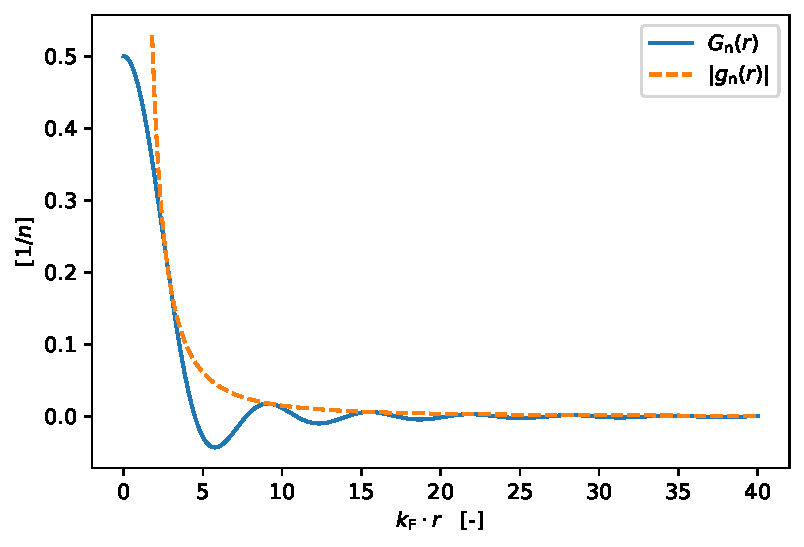
\includegraphics[width=10cm]{G_normal.pdf}
	\caption{A $G_\text{n}(\RR)$ és $\left| g_\text{n}(\RR) \right|$ függvények normált értéke $k_\text{F} r$ függvényében.}
	\label{G-normal-fig}
\end{figure}


\subsection{Szupravezető állapot járuléka}

\subsubsection{Az $F(\RR)$ függvény szupravezető járuléka}

Ugyanúgy, mint korábban itt is írjuk fel a \eqref{F-G-def} összefüggés alapján a szupravezető állapotban $F(\RR)$ értékét.  A számolás során felhasználjuk a \eqref{u-v-sc} értékeket, illetve a \eqref{cutoff} levágást.
\begin{equation}
\begin{split}
	F(\RR) & = \frac{1}{V} \sum\limits_\KK e^{-i \KK \RR} u_\KK v_\KK^* \approx \int \frac{\dd[3]k}{\left( 2 \pi \right)^3} ~ e^{-i \KK \RR} u_\KK v_\KK^* \cdot \frac{1}{\left( \frac{\xi_\KK}{\hbar \omega_\text{D}} \right)^4 + 1} = \\
	& = \int\limits_0^{2 \pi} \dd{\varphi} \int\limits_0^\pi \dd{\vartheta} \int\limits_0^\infty \frac{\dd{k}}{\left( 2 \pi \right)^3} ~ k^2 \sin\vartheta ~ e^{-i k r \cos\vartheta} \frac{\Delta^*}{2 \sqrt{\left| \Delta \right|^2 + \xi^2}} \cdot \frac{1}{\left( \frac{\xi}{\hbar \omega_\text{D}} \right)^4 + 1} = \\
	& = \frac{2}{\left( 2 \pi \right)^2} \, \frac{1}{r} \Im{ \int\limits_0^\infty \dd{k} ~ k \, e^{i k r} \frac{\Delta^*}{2 \sqrt{\left| \Delta \right|^2 + \xi^2}} \cdot \frac{1}{\left( \frac{\xi}{\hbar \omega_\text{D}} \right)^4 + 1} }
\end{split}
\end{equation}
Mivel a Fermi-felülethez közeli tartományon integrálunk, közelíthetjük a kitevőben lévő $k$ értékét az alábbi módon,
\begin{equation}
	k = \sqrt{\frac{2 m \left( E_\text{F} + \xi \right)}{\hbar^2}} \approx k_\text{F} + \frac{k_\text{F}}{2 E_\text{F}} \cdot \xi.
\end{equation}
A integrálban tényezőként lévő $k$ értékét egyszerűen $k_\text{F}$-el közelítjük, mert a pontosabb közelítésből csak egy elhanyagolható nagyságú korrekció származna.

Még érdemes bevezetni a $\Delta$ és $\hbar \omega_\text{D}$ energiákhoz tartozó hosszskálákat, a szupravezető korrelációs hosszat és a Debeye hullámhosszat,
\begin{equation}
	\xi_\text{c} \equiv \frac{2 E_\text{F}}{k_\text{F} \left| \Delta \right|} ~~~ \text{és} ~~~ \lambda_\text{D} \equiv \frac{2 E_\text{F}}{k_\text{F} \hbar \omega_\text{D}},
\end{equation}
illetve az $r$ és $\lambda_\text{D}$ viszonyított értékét a szupravezető korrelációs hosszhoz,
\begin{equation}
	\tilde{r} \equiv \frac{r}{\xi_\text{c}} ~~~ \text{és} ~~~ \tilde{\lambda}_\text{D} \equiv \frac{\lambda_\text{D}}{\xi_\text{c}}.
\end{equation}

Mindezeket felhasználva
\begin{equation}
	F(\RR) \approx \frac{2}{\left( 2 \pi \right)^2} \, \frac{k_\text{F}}{2 E_\text{F} r} \Im{ \int\limits_{-\infty}^\infty \dd{\xi} ~ k_\text{F} e^{i k_\text{F} r} e^{i \frac{k_\text{F}}{2 E_\text{F}} \xi \, r} \frac{\Delta^*}{2 \sqrt{\left| \Delta \right|^2 + \xi^2}} \cdot \frac{1}{\left( \frac{\xi}{\hbar \omega_\text{D}} \right)^4 + 1} }.
\end{equation}
Írjuk át az integrált az $x = \frac{\xi}{\left| \Delta \right|}$ változó szerint,
\begin{equation} \label{f-def}
	F(\RR) \approx \frac{2}{\left( 2 \pi \right)^2} \, \frac{k_\text{F}}{\xi_\text{c} r} \Im{ e^{i k_\text{F} r} \frac{\Delta^*}{\left| \Delta \right|} \int\limits_{-\infty}^\infty \dd{x} ~ e^{i \tilde{r} x} \frac{1}{2 \sqrt{1 + x^2}} \cdot \frac{1}{\left( \tilde{\lambda}_\text{D} x \right)^4 + 1} }.
\end{equation}
A továbbiakban jelöljük az integrált $I$-vel.  Ha az integrált kiterjesztjük a komplex síkra azt látjuk, hogy a $\sqrt{1 + x^2}$ miatt a komplex tengely mentén van egy szakadás, illetve az $\frac{1}{\left( \tilde{\lambda}_\text{D} x \right)^4 + 1}$ miatt négy pontban.  Az integrálási görbét transzformáljuk úgy, hogy a komplex tengely menti szakadást körülölelje.  Ekkor meg fog jelenni két reziduum $x_1 = \frac{i + 1}{\sqrt{2} \tilde{\lambda}_\text{D}}$ és $x_2 = \frac{i - 1}{\sqrt{2} \tilde{\lambda}_\text{D}}$ pontok körül.  Az integrálási változót írjuk át $x = i y$ szerint.  Így az integrál
\begin{equation}
	I = \int\limits_1^\infty \dd{y} ~ \frac{1}{\sqrt{y^2 - 1}} \, e^{-\tilde{r} y} \frac{1}{\left( \tilde{\lambda}_\text{D} y \right)^4 + 1} + R_1 + R_2,
\end{equation}
ahol $R_1$ és $R_2$ az $x_1$ és $x_2$ pont beli reziduumokat jelöli.

A reziddumokat könnyen felírhatjuk,
\begin{equation}
	R_1 = 2 \pi i \, e^{i \tilde{r} x_1} \frac{1}{2 \sqrt{1 + x_1^2}} \cdot \frac{1}{4 \tilde{\lambda}_\text{D}^4 x_1^3} \approx -\frac{i \pi}{4} \exp(i \frac{\tilde{r}}{\sqrt{2} \tilde{\lambda}_\text{D}}) \exp(-\frac{\tilde{r}}{\sqrt{2} \tilde{\lambda}_\text{D}})
\end{equation}
és
\begin{equation}
	R_2 = 2 \pi i \, e^{i \tilde{r} x_2} \frac{1}{2 \sqrt{1 + x_2^2}} \cdot \frac{1}{4 \tilde{\lambda}_\text{D}^4 x_2^3} \approx -\frac{i \pi}{4} \exp(-i \frac{\tilde{r}}{\sqrt{2} \tilde{\lambda}_\text{D}}) \exp(-\frac{\tilde{r}}{\sqrt{2} \tilde{\lambda}_\text{D}}).
\end{equation}
A kettő összege
\begin{equation}
	R_1 + R_2 \approx -\frac{i \pi}{2} \exp(-\frac{\tilde{r}}{\sqrt{2} \tilde{\lambda}_\text{D}}) \cos(\frac{\tilde{r}}{\sqrt{2} \tilde{\lambda}_\text{D}}).
\end{equation}

A komplex tengely menti integrál értékét vizsgáljuk meg $\tilde{r} \gg \tilde{\lambda}_\text{D}$ és $\tilde{r} \ll \tilde{\lambda}_\text{D}$ esetekben.  Távoltéri közelítésben az integrálból kihagyhatjuk a levágást, mivel az exponenciális rész sokkal gyorsabban vág le.  Ezzel az integrált kiszámolhatjuk,
\begin{equation}
	\int\limits_1^\infty \dd{y} ~ \frac{1}{\sqrt{y^2 - 1}} \, e^{-\tilde{r} y} = K_0(\tilde{r}),
\end{equation}
ahol $K_n(x)$ a másodfajú módosított Bessel-függvények.

Közeltéri közelítésben az integrálban lévő exponenciális függvényt sorba fejthetjük $\tilde{r}$ szerint,
\begin{multline}
	\int\limits_1^\infty \dd{y} ~ \frac{1}{\sqrt{y^2 - 1}} \left( 1 - \tilde{r} y \right) \frac{1}{\left( \tilde{\lambda}_\text{D} y \right)^4 + 1} = \\
	= \int\limits_1^\infty \dd{y} ~ \frac{1}{\sqrt{y^2 - 1}} \cdot \frac{1}{\left( \tilde{\lambda}_\text{D} y \right)^4 + 1} - \tilde{r} \int\limits_1^\infty \dd{y} ~ \frac{y}{\sqrt{y^2 - 1}} \cdot \frac{1}{\left( \tilde{\lambda}_\text{D} y \right)^4 + 1}.
\end{multline}
A kapott integrálokat numerikusan egyszerűen kiértékelhetjük.

A $G_\text{n}(\RR)$ számolásához hasonlóan itt is bevezethetünk egy $f(\RR)$ komplex mennyiséget, ami az $F(\RR)$ függvény burkolóját jellemzi.  A \eqref{f-def} összefüggés alapján felírhatjuk, hogy
\begin{equation}
	f(\RR) = \frac{2}{\left( 2 \pi \right)^2} \, \frac{k_\text{F}}{\xi_\text{c} r} \, \frac{\Delta^*}{\left| \Delta \right|} \cdot I.
\end{equation}


\subsubsection{$G(\RR)$ szupravezető járuléka}

\subsection{Asszimptotikus viselkedés}



% ================================================================
\section{Spin- és töltéskorrelációs függvények}

\subsection{Töltéskorreláció}
\subsection{Spinkorreláció}



\pdfbookmark{Hivatkozások}{bm:hivatkozasok}

\begin{thebibliography}{}
\end{thebibliography}


\end{document}
